\documentclass[11pt]{article}
\usepackage[small]{titlesec}
\usepackage[top = 0.66in,textwidth = 6.5in, textheight=9.1in]{geometry}

\usepackage{amsmath}
\usepackage{graphicx}
\usepackage{latexsym}
\usepackage{color}
\usepackage{amssymb}
\usepackage{tabularx}
\usepackage{fancyhdr}
\usepackage{verbatim}
\usepackage{multirow}
\usepackage{framed}
\usepackage{natbib}
\usepackage{float, subfig}
\usepackage{enumitem}
\usepackage{mathtools}
\usepackage{mathrsfs}
\usepackage{amsfonts}
\usepackage{listings}
\usepackage{amsthm}
\usepackage{grffile}
\usepackage{sidecap}
\usepackage{pbox}
\usepackage{algorithm}
\usepackage{longtable}
\usepackage[noend]{algpseudocode}

\def\qed{\hfill{\(\vcenter{\hrule height1pt \hbox{\vrule width1pt height5pt
     \kern5pt \vrule width1pt} \hrule height1pt}\)} \medskip}

\newtheorem{theorem}{Theorem}
\newtheorem{lemma}[theorem]{Lemma}
\newtheorem{corollary}[theorem]{Corollary}
\newtheorem{proposition}[theorem]{Proposition}
\newtheorem{conjecture}[theorem]{Conjecture}
\newtheorem{remark}{Remark}
\newtheorem{example}{Example}
\newtheorem{definition}{Definition}
\renewcommand{\textfraction}{0.0}
\newcommand{\dst}{\displaystyle}
\newcommand{\minx}{\mbox{\( \dst \min_{x \in X} \)}}
\newcommand{\Efx}{\mbox{\( \dst E f (x, \xi) \)}}
\newcommand{\Efxhat}{\mbox{\( \dst E f (\hat{x}, \xi) \)}}
\newcommand{\hxx}{\mbox{\( \hat{x} \)}}
\newcommand{\bpi}{\bar{\pi}}
\newcommand{\xx}{\mbox{\( x \)}}
\newcommand{\txxi}{\mbox{\(\xi\)}}
\newcommand{\var}{\mbox{var}}
\newcommand{\cF}{{\cal F}}
\newcommand{\cG}{{\cal G}}
\newcommand{\cN}{{\cal N}}
\newcommand{\cO}{{\cal O}}
\newcommand{\txi}{{\xi}}
\newcommand{\PP}{\mbox{\(SP\)}}
\newcommand{\PPn}{\mbox{\(SP_n\)}}
\newcommand{\PPnx}{\mbox{\(SP_{n_x}\)}}
\newcommand{\noi}{\noindent}
\renewcommand{\ss}{\smallskip}
\newcommand{\ms}{\medskip}
\newcommand{\bs}{\bigskip}
\newcommand{\st}{\mbox{s.t.}}
\newcommand{\wpo}{\mbox{wp1}}
\newcommand{\iid}{\mbox{i.i.d.\ }}
\newcommand{\vsmo}{\vspace*{-0.1in}}
\newcommand{\vsmt}{\vspace*{-0.2in}}
\newcommand{\vso}{\vspace*{0.1in}}
\newcommand{\vst}{\vspace*{0.2in}}
\newcommand{\mc}{\multicolumn}
\newcommand{\cP}{{\cal P}}
\newcommand{\underv}{\mbox{$\underbar{$v$}$}}
\allowdisplaybreaks 

\renewcommand{\P}{{\mathbb P}}
\newcommand{\E}{{\mathbb E}}
\newcommand{\R}{{\mathbb R}}
\renewcommand{\Re}{{\mathbb R}}
\newcommand{\mbf}{\mathbf}

\bibliographystyle{plain}

\begin{document}
%0.27
\baselineskip0.25in

\begin{center}
\begin{large}
\begin{bf}

Optimizing Crashing Decisions in Project Management Problem with Disruptions \ms

\today \ms
\end{bf}
\end{large}
\end{center}

\section{Introduction} \label{sec:introduction}
	Project management has been a topic studied by many operations researchers using ``engineering science and optimization theory" \cite{soderlund2004building}. In order to derive an abstract model, a project could be viewed as a collection of activities, each of which will consume some time and resources. There will be precedence relationships between activities due to logical or technological considerations. The objective is to find the smallest amount of time needed to finish all activities. The project could be represented as an activity network where the length of each link shows the duration of an activity, and the direction of it shows the precedence relationship. An activity cannot start until all its predecessors are completed. Two dummy nodes \((S,T)\) are created in the network to represent the start and the end of the project. In the network setting with no uncertainty, finding the shortest project span is equivalent to finding the longest path from \(S\) to \(T\). Since the activity network is usually acyclic, it is easy to use shortest path algorithms to find a longest path in polynomial time. Multiple projects can be processed at the same time without a upper limit, as long as the precedence requirement is satisfied. More details about the activity network are discussed in \cite{Elmaghraby77}.\\
	\newline 
	In the planning stage of a project, decisions can be made to crash a certain set of activities in order to achieve the shortest project span. Here crashing an activity means accelerating its progress or compress its duration. In this paper, a discrete set of crashing options will be given to the decision makers, each with a fractional number which equals to the crashed duration divided by the original duration. One project can only be crashed once with one specific option. Each option will incur a certain cost as well and the total cost of crashing could not exceed the budget. Static crashing optimization problem is first researched in \cite{fulkerson1961network, kelley1961criticalpath}. If we assume a finite set of crashing options, the problem could be modeled as a mixed integer program. The static model can be extended to incorporate uncertainty of activity durations. Monte Carlo simulation methods are used to estimate the expected project span given distributions of activity lengths, since it is not really possible to provide an analytical expression of the true expected project span \cite{burt1971conditional,van1963letter}. Heuristics and simulation-based algorithms have been developed to solve the stochastic project crashing problem \cite{aghaie2009ant,bowman1994stochastic,ke2014genetic,kim2007heuristic}. Another approach to handle the uncertainty is the robust optimization method. In the robust optimization setting, the objective is to minimize the worst case project span within the uncertainty set. It can be proved that an affinely adaptive recourse decision, although computationally tractable as it can be reformulated as a linear program or a second order conic program (SOCP), may lead to suboptimal solutions \cite{chen2008linear,cohen2007stochastic}. However, once the recourse decision rule is extended to a general form, it is only tractable to solve the robust optimization problem with hypercube uncertainty sets, which is a trivial case because the worst-case scenario in the uncertainty set is always the point where every activity takes the upper bound. \cite{wiesemann2012robust}. In recent years, distributionally robust optimization has been developed quickly in literature \cite{delage2010distributionally}. Ahipasaoglu et al. \cite{ahipasaoglu2016distributionally} propose a distributionally robust optimization scheme applied to PERT network, which reformulates the problem as a semidefinite program or a copositive program, depending on the description of uncertainty.\\
	\newline
	The uncertainty in our paper lies in the timing and the magnitude of the stochastic disruption, which is modeled in a different way from the random variable distribution in the stochastic programming setting, or from the uncertainty set in the robust optimization setting. A stochastic disruption is an event that may occur any time in the time horizon and change the system parameters significantly. There have been a few papers in applying this idea when the disruption could only occur in a set of specified time periods. Yu and Qi \cite{yu2004disruptionmgt} introduced scenario-based optimization models and applied it to solve airline scheduling problems. Morton et al. \cite{morton2009sealift} introduced the modeling of a sealift scheduling problem under finite number of stochastic disruptions within a stochastic programming structure. This structure ``falls between standard two-stage and multi-stage stochastic programs for a multi-period problem" and reduces the size of the problem to a quadratic growth in the number of time periods. Our setting inherits the philosophy of \cite{morton2009sealift} but enhances the model by allowing continuous disruption time instead of fixed time periods.\\
	\newline
	We first formally describe the crashing optimization problem under stochastic disruptions. Given the limited number of disruption occurrence, the problem can be formulated as a stochastic mixed integer program and we will present the extensive formulation in Section~\ref{sec:formulation}. If we assume continuous distributions for the disruption time and magnitude, sample average approximation (SAA) can be used to create a finite set of scenarios and approximate the original problem by a finite-sized optimization problem. We prove some important consistency and convergence properties of the SAA problem using independent and identically distributed samples and stratified samples in Section~\ref{sec:consistency}.\\
	\newline
	The large scale and the discrete non-convex nature of the SAA problem's extended formulation means it may not be solved efficiently to desirable tolerance level. In Section~\ref{sec:decomposition}, a branch-and-cut method based on Benders decomposition is developed to solve the crashing optimization problem with a disruption. We show such a decomposition method will solve the integer program to the exactness within finite number of iterations.\\
	\newline
	The experiment results are presented in Section~\ref{sec:results}, including the comparison between the quality of our solution and the solution obtained by solving a  crashing optimization problem with a deterministic disruption, and the computational performance of the decomposition method in Section~\ref{sec:decomposition}, compared to that of solving the extensive formulation. We will conclude our paper with remarks on potential extensions of this model in Section~\ref{sec:conclusions}.
	
\section{Problem Formulation} \label{sec:formulation}
	The deterministic project crashing optimization problem is widely researched since 1960s \cite{fulkerson1961network, kelley1961criticalpath}. Suppose the activity network is represented by a directed graph \(\mathcal{G} = (I,\mathcal{A})\), where the set of activities is denoted by \(I\) and their precedence relationship is characterized by \(\mathcal{A}\). The budget limit \(B\) and the nominal length of each activity \(D_i\) are given. For each activity \(i \in I\), there is a finite set of crashing options \(j \in J_i\) and each of them will incur a cost of \(b_{ij}\) while cutting down the nominal activity length to \(1 - e_{ij}\) of the nominal length.  We assume each activity could be crashed at most once and the problem could be formulated as follows. 
	\begin{subequations} \label{prob2:static}
		\begin{align}
		\min \quad & t_N &\\
		\text{s.t.} \quad & t_N \geq t_i & \forall \,i \in I \\
		& t_k - t_i \geq D_{i}(1 - \sum_{j \in J_i} x_{ij} e_{ij}) & \forall \,i \in I, (i,k) \in \mathcal{A}\\
		& \sum_{i \in I} \sum_{j \in J_i} b_{ij}x_{ij} \leq B & \\
		& \sum_{j \in J_i} x_{ij} \leq 1 & \forall \,i \in I\\
		& t_i \geq 0 & \forall \,i \in I\\
		& 0 \leq x_{ij} \leq 1 & \forall \,i \in I, j \in J_i&
		\end{align}
	\end{subequations}
	Based on this formulation, we can derive the stochastic optimization and the robust optimization models with reference to the literature listed in Section~\ref{sec:introduction}. We omit these formulations in this paper since our uncertainty model is different from previous settings.\\
	\newline
	We assume at most one stochastic disruption will occur in the project span. The disruption will not affect the activities that have already started but will change the length of activities starting after it according to some given finite discrete distributions. The decision of crashing has to be made the same time when the activity starts and cannot be changed after that. Since there is at most one disruption, we can model the problem as a two-stage stochastic mixed integer program. Notice that the definition of the first stage is different from the traditional stochastic program setting. Here the first stage contains all the decisions if no disruption occurs and the second stage will characterize the decisions for each realization of the disruption. This means that the first stage decision variables are not limited to a certain time period but can be all over the entire time horizon, which allows us to model continuous disruption time.\\
	\newline
	The notation for the model is displayed as follows:
	\begin{longtable}[H]{ l l l l }
		\multicolumn{4}{l}{Indices and index sets} \\
		\\
		\(I\) & \(\qquad\) & the set of activities;&\\
		\(I_i\) & \(\qquad\) & the set of activities which directly lead to activity \(i\); &\\
		\(J_i\) & \(\qquad\) & the set of crashing options for activity \(i\), \(i \in I\);&\\
		\(\Omega\) & \(\qquad\) & the set of possible realizations of disruption;&\\
		\(\mathcal{A}\) &\(\qquad\) & set of arcs which represents the precedence relationship;&\\
		\\
		\multicolumn{4}{l}{Parameters} \\
		\\
		\(D_{i}\)& \(\qquad\) & original duration of activity \(i\), \(i \in I\);&\\
		\(e_{ij}\) & \(\qquad\) & effectiveness of crashing option \(j\), \(i \in I, j \in J_i\);&\\
		\(B\) & \(\qquad\) & total budget;&\\
		\(b_{ij}\) & \(\qquad\) & cost of crashing option \(j\), \(i \in I, j \in J_i\);&\\
		\(H^\omega\) &\(\qquad\) & disruption time in scenario \(\omega\), \(\omega \in \Omega\);&\\
		\(d_{i}^\omega\) & \(\qquad\)&the change of duration of activity \(i\) in realization \(\omega\), &\\
		& \(\qquad\) & if the activity is started after the disruption, \(i \in I, \omega \in \Omega\);& \\
		\(p^\omega\) & \(\qquad\) & the probability of scenario \(\omega\), \(\omega \in \Omega\);& \\
		\(p^0\) & \(\qquad\) & the probability of no disruption;& \\
		\\
		\multicolumn{4}{l}{Decision Variables}\\
		\\
		\(t_{i}\) & \(\qquad\) & nominal starting time of activity \(i\), \(i \in I\);&\\
		\(x_{ij}\) & \(\qquad\) & indicator whether activity \(i\) is crashed by option \(j\) in the nominal plan, \(i \in I, j \in J_i\); &\\
		\(t_{i}^\omega\) & \(\qquad\) & starting time of activity \(i\) under scenario \(\omega\), \(i \in I, \omega \in \Omega\);&\\
		\(x_{ij}^\omega\) & \(\qquad\) & indicator whether activity \(i\) is crashed by option \(j\) under scenario \(\omega\), \(i \in I, j \in J_i, \omega \in \Omega \); &\\
		\(G_i^\omega\) & \(\qquad\) & indicator whether activity \(i\) starts after disruption in realization \(\omega\), \(i \in I, \omega \in \Omega\);&\\
		\(S_{ij}^\omega\) & \(\qquad\) & binary term to linearize the bilinear term \(G_i^\omega x_{ij}^\omega\), \(i \in I, j \in J_{i}, \omega \in \Omega\).&\\
	\end{longtable}
	\noi The extensive formulation of the two-stage stochastic program is shown as Formulation~(\ref{prob2:extensive}). Here \(M\) is a large number to enforce the logic relationships. In this problem, we are minimizing the expected project span by taking the sum of each scenario's project span weighted by the scenario probability. Variables \(G^\omega_i\) are used to identify whether activity \(i\) starts before or after the disruption time (in constraint (\ref{cons:F}) - (\ref{cons:G})). This is important in our problem setting because the duration of each activity will depend on its temporal relationship to the disruption time, which is reflected in constraint (\ref{cons:duration}). For this duration constraint, the original expression of the duration of activity \(i\) is \((D_i + d_i^\omega G_i^\omega)(1 - \sum_{j \in J_i} e_{ij}x_{ij}^\omega)\). This contains a bilinear term \(G_i^\omega x_{ij}^\omega\), which can be linearized by introducing a binary variable \(S_{ij}^\omega\) and bounding it by constraints (\ref{cons:linearize1}) - (\ref{cons:linearize3}).\\
	\newline
	We have to use a set of non-anticipativity constraints (\ref{cons:tf1}) - (\ref{cons:xf2}), different from the one used in a traditional stochastic programming setting, since the first stage decision variables here spans the entire time horizon. These logic constraints ensure the decisions made before the disruption time in each scenario should be the same as the nominal decisions before the same time point, because decisions made with the same amount information should be the same.\\
	\begin{subequations} \label{prob2:extensive}
		\begin{align}
		\min \quad & \sum_{\omega \in \Omega} p^\omega t_N^\omega + p^0 t_N& \\
		\text{s.t.} \quad & t_N^\omega \geq t_i^\omega & \forall \,i \in I, \omega \in \Omega \\
		& t_N \geq t_i & \label{cons:tN}\\
		& t_i^\omega \geq 0 & \forall \,i \in I, \omega \in \Omega\\
		& t_i \geq 0 & \forall \,i \in I\\
		& H^\omega - (1 - G_i^\omega) M \leq t_i & \forall \,i \in I, \omega \in \Omega \label{cons:F}\\
		& H^\omega + G_i^\omega M \geq t_i & \forall \,i \in I, \omega \in \Omega \label{cons:G}\\
		& t_i^\omega + G_i^\omega M \geq t_i & \forall \,i \in I, \omega \in \Omega \label{cons:tf1}\\
		& t_i^\omega - G_i^\omega M \leq t_i & \forall \,i \in I, \omega \in \Omega \label{cons:tf2}\\
		& x_{ij}^\omega + G_i^\omega \geq x_{ij} & \forall \,i \in I, j \in J_i, \omega \in \Omega \label{cons:xf1}\\
		& x_{ij}^\omega - G_i^\omega \leq x_{ij} & \forall \,i \in I, j \in J_i, \omega \in \Omega \label{cons:xf2}\\
		& t_k^\omega - t_i^\omega \geq D_i + d_i^\omega G_i^\omega -\sum_{j \in J_i} D_i e_{ij} x_{ij}^\omega - \sum_{j \in J_i} d_i^\omega e_{ij} S_{ij}^\omega & \forall \,i \in I, j \in J_i, \omega \in \Omega \label{cons:duration}\\
		& \sum_{j \in J_i} x_{ij}^\omega \leq 1 & \forall \,i \in I, \omega \in \Omega \label{cons:crashLim}\\
		& \sum_{i \in I}\sum_{j \in J_i} b_jx_{ij}^\omega \leq B & \forall \,\omega \in \Omega \label{cons:budget}\\
		& S_{ij}^\omega \leq G_i^\omega & \forall \,i \in I, j \in J_i, \omega \in \Omega \label{cons:linearize1}\\
		& S_{ij}^\omega \leq x_{ij}^\omega & \forall \,i \in I, j \in J_i, \omega \in \Omega \label{cons:linearize2}\\
		& S_{ij}^\omega \geq G_i^\omega + x_{ij}^\omega - 1 & \forall \,i \in I, j \in J_i, \omega \in \Omega \label{cons:linearize3}\\
		& t_i \geq 0 & \forall\,i \in I \\
		& t_i^\omega \geq H^\omega G_i^\omega & \forall\, i \in I, \omega \in \Omega \\
		& 0 \leq x_{ij} \leq 1 & \forall \,i \in I, j \in J_i\\ 
		& 0 \leq x_{ij}^\omega \leq 1 & \forall \,i \in I, j \in J_i, \omega \in \Omega\\
		& G_i^\omega \in \{0,1\}. & \forall \,i \in I, \omega \in \Omega
		\end{align}
	\end{subequations}

\section{Special Cases} \label{sec:examples}
	In this section we show a few examples to illustrate the properties of the project crashing problem under stochastic disruption displayed in Section~\ref{sec:formulation}. We will focus on simple network structures such as serial and parallel networks. We also display some general networks where those properties are (or not) applicable.
	\subsection{Serial Networks}
		\begin{itemize}
			\item Concavity of \(\mathbb{E}_d \left[ f(x,H,d) | H \right]\) in \(d\).
			\item The recourse function is a decreasing function in terms of remaining budget, given the same remaining task set.
			\item Not optimal to delay the start of activity \(i\) unless there is no investment before \(i\), given a fixed \(H\).
			\item Only optimal to delay to a possible disruption time.
		\end{itemize}
		The first example we present for a serial network is to show that it might be optimal to delay the start of some activities. The reasons of such delay include:
		\begin{enumerate}
			\item Some activities might have a shorter length after disruption. It is beneficial to wait a short period of time to capture this advantage.
			\item Even if all possible disruption magnitudes are adverse, which means they will lengthen all activities, it is beneficial to delay an activity so that the crashing resource could be optimally applied according to the realization of disruption.
		\end{enumerate}
		Suppose we have a project with three activities in a serial network form. The activity 1 should be finished before the start of activity 2 and the activity 2 should be finished before the start of activity 3. The structure of the project is displayed as follows. We add two dummy activity ``S" and ``T" to represent the start and the end of the project. The total crashing budget is \(1\) and the allowed amount of crashing a single activity is between \(0\) and \(1\). 
		\begin{figure}[H]
			\centering
			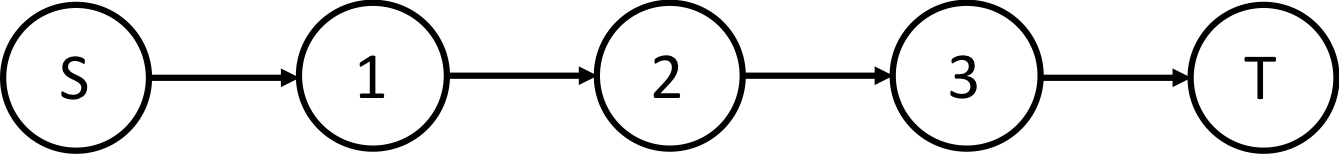
\includegraphics[width=0.8\textwidth]{serial3}
			\caption{Example of a 3-activity project}
			\label{fig:serial3}
		\end{figure}
		\noi We can set up a nominal case with the length of activity 1, 2 and 3 as \(9\), \(10\) and \(7\). The probability of the disruption not occurring is 0.5. If a disruption occurs, it will occur at the time \(H = 9.1\). Suppose the disruption will change the length of activity 2 from \(10\) to \(3\) and not affect activity 3. We can see it is optimal to delay the start of activity 2 to \(t_2 = 9.1\), spend the entire budget to crash activity 3 if the disruption occurs, and spend the entire budget to crash activity 2 if the disruption does not occur. The expected total project span is 18.35. If we force the condition that the starting time of activities could not be delayed, we could not observe whether the disruption happens or not at the starting time of activity 2. There will be only one possible situation where three activities will have the duration as 9,10 and 7. All resources should be allocated to activity 2 and the total project span is 21, which is larger than the expected total project span if it is allowed to delay the starting time of some activities. The reason of such phenomenon is that a disruption may reduce some activities' durations. Delaying by a small amount will enable us to collect that reduction in time.\\
		\newline
		Even if the disruption can only bring negative effect on the duration of activities, a.k.a. lengthening all activities after that, it is still beneficial to delay the start of some activities under some circumstances. This means a small delay of some activity may gain the information of disruption which is more valuable and potentially decreases the total project span. Such claim can be verified by the serial network described in the last paragraph, only changing some duration parameters in the following way. Suppose the nominal duration, the timing of possible disruption and the probability of a disruption occurring remain the same. If the disruption occurs, it will change the duration of activity 2 to 9.1 and that of activity 3 to 13. For this example, if no delay is allowed, the optimal decision is to allocate the entire budget to activity 2 and the expected total project span is 24. If we delay the starting time of the activity 2 to 9.1 so that the disruption can be observed before we commit resources to activity 2, the expected total project span is 23.4. 
	\subsection{Parallel Networks}
		\begin{itemize}
			\item Not optimal to delay when \(d_i \geq 0\).
		\end{itemize}
	\subsection{Y Networks}
\section{Properties of the Sample Average Approximation Problem} \label{sec:consistency}
	\subsection{Cheat?}
	\subsection{Consistency and Convergence Results}
	\subsection{IID vs. Stratified Sampling}
\section{Decomposition Method} \label{sec:decomposition}
	Problem~\eqref{prob2:extensive} is a two-stage stochastic mixed integer program with binary variables in the second stage. 
\section{Experiment Results} \label{sec:results}
	\subsection{Deterministic Counterparts}
		List the test results of INFORMS presentation. State the fact that the fully stochastic makes great improvement over its deterministic counterparts.
\section{Stochastic Mixed Integer Program Extension}
\section{Conclusions} \label{sec:conclusions}

\bibliographystyle{plain}
\bibliography{PERT_Bib}

\end{document}